\begin{comment}

\lstset{width=\textwidth,
          %frame = single,
          escapechar=@,
          language=SQL,
          basicstyle=\scriptsize
          }

\newsavebox{\firstlisting}
\begin{lrbox}{\firstlisting}% Store first listing
\begin{lstlisting}
select c_count, count(*) as custdist
from ( select c_custkey, count(o_orderkey)
       from customer left outer join orders on 
       c_custkey = o_custkey and 
       o_comment not like '%pending%accounts%'
       group by c_custkey
      ) as c_orders (c_custkey, c_count)
group by c_count
order by custdist desc, c_count desc;
\end{lstlisting}
\end{lrbox}

\newsavebox{\secondlisting}
\begin{lrbox}{\secondlisting}% Store first listing
\begin{lstlisting}
select p_brand, p_type, p_size,
        count(distinct ps_suppkey) as supplier_cnt
from partsupp, part
where p_partkey = ps_partkey
        and p_brand <> 'Brand#35'
        and p_type not like 'ECONOMY BURNISHED%'
        and p_size in (14, 7, 21, 24, 35, 33, 2, 20)
        and ps_suppkey not in ( select s_suppkey
            from supplier
            where s_comment like '%Customer%Complaints%')
group by p_brand, p_type, p_size
order by supplier_cnt desc, p_brand, p_type, p_size;

\end{lstlisting}
\end{lrbox}

\newsavebox{\thirdlisting}
\begin{lrbox}{\thirdlisting}% Store first listing
\begin{lstlisting}
select sum(l_extendedprice* (1 - l_discount)) as revenue
from lineitem, part
where
 ( p_partkey = l_partkey and p_brand = 'Brand#23'
    and p_container in ('SM CASE', 'SM BOX', 'SM PACK', 'SM PKG')
    and l_quantity >= 5 and l_quantity <= 5 + 10
    and p_size between 1 and 5 and l_shipmode in ('AIR', 'AIR REG')
    and l_shipinstruct = 'DELIVER IN PERSON' )
or 
(  p_partkey = l_partkey and p_brand = 'Brand#15'
   and p_container in ('MED BAG', 'MED BOX', 'MED PKG', 'MED PACK')
   and l_quantity >= 14 and l_quantity <= 14 + 10
   and p_size between 1 and 10 and l_shipmode in ('AIR', 'AIR REG')
   and l_shipinstruct = 'DELIVER IN PERSON')
or 
( p_partkey = l_partkey and p_brand = 'Brand#44'
   and p_container in ('LG CASE', 'LG BOX', 'LG PACK', 'LG PKG')
   and l_quantity >= 28 and l_quantity <= 28 + 10
   and p_size between 1 and 15 and l_shipmode in ('AIR', 'AIR REG')
   and l_shipinstruct = 'DELIVER IN PERSON' );
\end{lstlisting}
\end{lrbox}


\begin{figure*}[ht]
\sbox{\measurebox}{
\begin{minipage}[b]{.33\textwidth}
\subfloat[Q13]{\usebox{\firstlisting}}
\hfill%
\subfloat[Q16]{\usebox{\secondlisting}}  
\end{minipage}
}
\usebox{\measurebox}\qquad
\hspace{4em}
\begin{minipage}[b][\ht\measurebox][s]{.33\textwidth}
\subfloat[Q19]{\usebox{\thirdlisting}} 
\end{minipage}
\caption{ Queries}
\label{fig:queries}
\end{figure*}


\end{comment}

\section{Simulation Testbed}
This section details our experimental settings in terms of the hardware
parameters, the database and query workload, and the performance metrics
on which we evaluated the algorithms.

\label{sec:exp}


\subsection{Architectural Platform}
Since PCM memory is as yet not commercially available, we
have taken recourse to a simulated hardware environment to
evaluate the impact of the PCM-conscious operators.  For this
purpose, we chose Multi2sim~\cite{multi2sim}, an open source
application-only\footnote{Simulates only the application layer without
the OS stack.} simulator that can model a multithreaded, multicore,
superscalar x86 CPU and an AMD Evergreen GPU. It has support for both
functional simulation and cycle-accurate detailed architecture simulation.

We evaluated our algorithms on Multi2sim in cycle-accurate simulation
mode. Since it does not have native support for PCM, we made a major
extension to its existing memory module to model PCM memory. Specifically,
the following enhancements were incorporated in the simulator to conduct
our experimental evaluation:

\textbf{Hybrid Main Memory}: 
The memory organization was extended such that the new configuration
consists of PCM with a hardware controlled DRAM buffer. The DRAM buffer
acts as another level of cache in the memory hierarchy, specifically
between the L2 cache and the PCM.

\\\textbf{New DRAM Replacement Policy}: 
The DRAM is simulated as a set-associative write-back memory with
\textit{N-Chance} as the eviction policy. As mentioned in \cite{nchance},
$N$ was set to $\frac{K}{2}$, where $K$ is the cache associativity,
since this setting was found to provide good performance on multiple
metrics -- writes, energy and latency.

\\\textbf{Tracking DRAM-PCM Data}:
Like most other architectural simulators, Multi2sim does not explicitly
track the data residing at the different levels of the memory
hierarchy. It instead maintains only a single buffer that indicates
the latest data, as visible to the simulated program, for each memory
location. We therefore had to add separate data tracking functionality
for the DRAM and PCM resident data.

\\\textbf{Data Comparison Write Scheme}: 
The write-back mechanism of data from DRAM to PCM was modelled on the
DCW~\cite{write} scheme. Thus, for each evicted DRAM block, a comparison
to the original PCM resident data block was made, and writes were
restricted to only those words where the data bits differed. In our
experiments, we measured writes at \textit{word} (4B) granularity.

\\\textbf{Asymmetric Read-Write Latencies}:  
The timing simulation was modified to account for the higher write
latency of PCM as compared to a read.

\\\textbf{Wear Distribution}: 
Apart from the raw number of writes, a critical related metric for PCM
algorithms is their wear distribution. We therefore instrumented the
Multi2sim code to track block level wear distribution information. To
achieve this, separate counters were created that tracked writes to each
PCM \textit{line} (256B) during the query processing activity.

\\\textbf{Intermediate Statistics}: 
Multi2sim does not have support to track intermediate statistics during
a program run. We therefore provided additional inter-process communication capabilities in the
tool so that the simulated program could ask the simulator to dump
statistics for each intermediate operator during the execution of a query.

\begin{center}
\begin{table}[htbp]
\begin{small}
\caption{Experimental Setup}
\label{table:setup}
\begin{tabular}{p{2.5cm}p{10cm}}
\toprule
Simulator & Multi2sim-4.2 with added support for PCM\\ \hline

L1D cache (private) & 32KB, 64B line, 4-way set-associative, 4 cycle latency, write-back, LRU replacement policy\\ \hline
L1I cache (private) & 32KB, 64B line, 4-way set-associative, 4 cycle latency, write-back, LRU replacement policy\\ \hline   
L2 cache (private) & 256KB, 64B line, 4-way set-associative, 11 cycle latency, write-back, LRU replacement policy\\ \hline

DRAM buffer (private) & 4MB, 256B line, 8-way set-associative, 200 cycle latency, write-back, N-Chance replacement policy (N = 4)\\ \hline

Main Memory & 2 GB PCM, 4KB page, 1024 cycle read latency (per 256B line), 64 cycle write latency (per 4B modified word)\\
\bottomrule
\end{tabular}
\end{small}
\end{table}
\end{center}


The specific configurations used in the memory hierarchy (L1 Data,
L1 Instruction, L2, DRAM Buffer, PCM) evaluated in our experiments are
enumerated in Table~\ref{table:setup}.  These values are scaled down
versions, wrt number of lines, of the hardware simulation parameters used
in \cite{wear} -- the reason for the scaling down is to ensure that the
simulator running times are not impractically long. However, we have been
careful to ensure that the \emph{ratios} between the sizes of adjacent
levels in the hierarchy are maintained as per the original configurations
in \cite{wear}.  
\begin{comment}
Further, note that the read-to-write latency ratio is
1:4, significantly lower than the 1:20 of Table ~\ref{tab:tab_pcm_char}
in the Introduction. We wish to point out that this makes our results
\emph{conservative} -- if the ratio is made 1:20, the performance
improvements of the new algorithms  are even more substantial.
\end{comment}

Finally, despite the Multi2sim simulator having support for multiple
threads/processes, we restricted our experiments to a single process with
a single thread of execution. This choice ensured that the entire private
DRAM was available to the executing query. The effect of reduced DRAM
availability due to multiple programs running in parallel was \emph{inferred}
by conducting additional experiments with reduced DRAM sizes, and 
these results are presented in the Appendix.
\begin{figure*}[htpb]
\centering
\subfloat[Q13]{
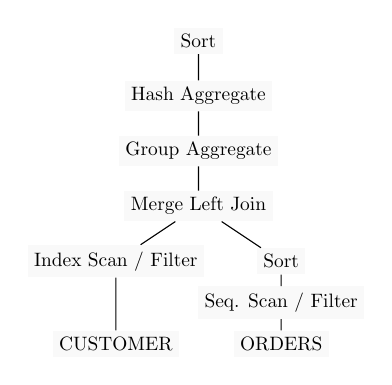
\begin{tikzpicture}[scale=.7, transform shape]

\tikzstyle{every node} = [rectangle, fill=gray!5]

\node (d) at (0,3) {Index Scan / Filter};
\node (c) at (0,1.5) {CUSTOMER};

\node (s) at (3,3) {Sort};
\node (p) at (3,2.25) {Seq. Scan / Filter};
\node (a) at (3,1.5) {ORDERS};

\node (e) at (1.5,4) {Merge Left Join};
\node (f) at (1.5,5)  {Group Aggregate};
\node (g) at (1.5,6)  {Hash Aggregate};
\node (h) at (1.5,7)  {Sort};


\draw[-] (c) -- (d);
\draw[-] (a) -- (p);
\draw[-] (d) -- (e);
\draw[-] (p) -- (s);
\draw[-] (s) -- (e);
\draw[-] (e) -- (f);

\draw[-] (f) -- (g);
\draw[-] (g) -- (h);

\end{tikzpicture}
}
\subfloat[Q16]{
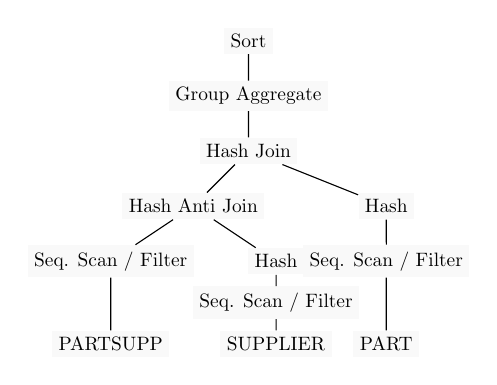
\begin{tikzpicture}[scale=.7, transform shape]

\tikzstyle{every node} = [rectangle, fill=gray!5]

\node (d) at (0,3) {Seq. Scan / Filter};
\node (c) at (0,1.5) {PARTSUPP};

\node (s) at (3,3) {Hash};
\node (p) at (3,2.25) {Seq. Scan / Filter};
\node (a) at (3,1.5) {SUPPLIER};

\node (e) at (1.5,4) {Hash Anti Join};

\node (n) at (5, 4) {Hash};
\node (b) at (5,3) {Seq. Scan / Filter};
\node (x) at (5,1.5) {PART};

\node (f) at (2.5,5)  {Hash Join};
\node (g) at (2.5,6)  {Group Aggregate};
\node (h) at (2.5,7)  {Sort};


\draw[-] (c) -- (d);
\draw[-] (a) -- (p);
\draw[-] (d) -- (e);
\draw[-] (p) -- (s);
\draw[-] (s) -- (e);
\draw[-] (e) -- (f);

\draw[-] (x) -- (b);
\draw[-] (b) -- (n);
\draw[-] (n) -- (f);

\draw[-] (f) -- (g);
\draw[-] (g) -- (h);

\end{tikzpicture}

}
\subfloat[Q19]{


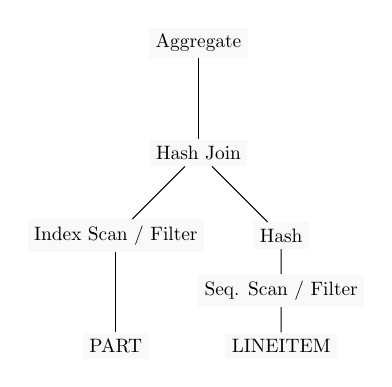
\begin{tikzpicture}[scale=.7, transform shape]

\tikzstyle{every node} = [rectangle, fill=gray!5]

\node (d) at (0,3.5) {Index Scan / Filter};
\node (c) at (0,1.5) {PART};

\node (s) at (3,3.5) {Hash};
\node (p) at (3,2.5) {Seq. Scan / Filter};
\node (a) at (3,1.5) {LINEITEM};

\node (e) at (1.5,5) {Hash Join};
\node (f) at (1.5,7)  {Aggregate};


\draw[-] (c) -- (d);
\draw[-] (a) -- (p);
\draw[-] (d) -- (e);
\draw[-] (p) -- (s);
\draw[-] (s) -- (e);
\draw[-] (e) -- (f);
\end{tikzpicture}
}

\caption{ Query execution plan trees}

\label{fig:plan_trees}

\end{figure*}

%\vspace*{0.05in}

\subsection{Database and Queries}
%We used TPC-H (version 2.16.0) 1GB PCM-resident database for our experiments.
For the data, we used the default 1GB database generated by the TPC-H
benchmark.  This size is certainly small compared to the database sizes
typically encountered in modern applications -- however, we again chose
this reduced value to ensure viable simulation running times.

\begin{comment}
Notwithstanding, to ensure that our results were not skewed 
as an outcome,  we used scaled down versions of the hardware simulation parameters
from \cite{wear}, taking care to preserve the size ratios between adjacent
memory devices.
\end{comment}

For simulating our suite of database operators -- \textit{sort},
\textit{hash join} and \textit{group by} -- we created a separate library
consisting of the native PostgreSQL implementation of these operators. To
this library, we added the PCM-conscious versions described in the
previous sections.

While we experimented with several of the TPC-H queries, results for
three queries: Query 13 (Q13), Query 16 (Q16) and Query 19 (Q19), that
cover a diverse spectrum of the experimental space, are presented here.
For each of the queries, we first identified the query execution plan
recommended by the PostgreSQL query optimizer with the native operators,
and then forcibly used the same execution plan for their PCM-conscious
replacements as well. This was done in order to maintain fairness in the
comparison of the PCM-oblivious and PCM-conscious algorithms, though it
is possible that a better plan is available -- we return to this issue 
later in Section~\ref{discussion}. 
%The three SQL queries are enumerated in Figure~\ref{fig:queries}, and their associated execution plans are shown in Figure~\ref{fig:plan_trees}.
The execution plans associated with the three queries are shown in Figure~\ref{fig:plan_trees}. 
 







\subsection{Performance Metrics}
We measured the following performance metrics for each of the queries:
\begin{description}
\item [PCM Writes:] This is the total number of word (4B) updates that are applied to the PCM memory during
the query execution.
\jhcomment{important to write correctly}
\item [CPU Cycles:] This is the total number of CPU cycles requires to execute the query to completion.
\item [Wear Distribution:] This is the frequency of writes measured on a per-256B-block basis.
\end{description}
To aid in understanding the global performance represented by the above metrics, we also drilled
down and measured the writes and cycles on a \emph{per-operator} basis during the query
execution.


\section{Experimental Results}
\label{sec:results}
Based on the above framework, we conducted a wide variety of experiments
and present a representative set of results in this section.

We begin by profiling the PCM Writes and CPU Cycles behavior of
the native and PCM-conscious executions for Q13, Q16 and Q19 --
these results are shown in Figures~\ref{fig:overall_results_q13},
\ref{fig:overall_results_q16} and \ref{fig:overall_results_q19},
respectively.  In each of these figures, we provide both the total and
the break-ups on a per operator basis.

\begin{figure}[htbp]
\centering
  	\includegraphics[height=29mm]{overall_q13.png}
	\caption{Impact of sort on overall performance - Q13}
	\label{fig:overall_results_q13}
\end{figure}

Focusing our attention first on Q13 in
Figure~\ref{fig:overall_results_q13}, we find that the bulk of the
overall Writes and Cycles are consumed by the Sort operator. Comparing
the performance of the Native (blue bar) and PCM-conscious (green bar)
implementations, we observe a very significant savings (53\%) on Writes,
and an appreciable decrease (20\%) on Cycles.

\begin{figure}[htbp]
	\centering
	\includegraphics[height=29mm]{overall_q16.png}
	\caption{Impact of group-by on overall performance - Q16}
	\label{fig:overall_results_q16}
\end{figure}
Turning our attention to Q16 in Figure~\ref{fig:overall_results_q16},
we find that here it is the group-by operator that primarily influences
the overall Writes performance, whereas the hash-join determines the
Cycles behavior. Again, there are substantial savings in both Writes
(40\%) and  Cycles (30\%) delivered by the PCM-conscious approach.

\begin{figure}[htbp]
	\centering
 	\includegraphics[height=29mm]{overall_q19.png}
	\caption{Impact of hash join on overall performance - Q19}
	\label{fig:overall_results_q19}
\end{figure}



\begin{comment}
In case of Q13, the running time and writes for the sort operator formed
the bulk of the writes and time taken for the entire query. The group-by
operator comparatively incurred negligible writes and running time. Writes
savings of 53\% and running time savings of 20\% were observed for the
execution of Q13 (shown in sub-figures (a) and (b) resp.) as compared
to native; fuelled mainly by the sort operator.
\end{comment}



\begin{comment}
In case of Q16, both the group-by and hash join operators incurred
significant writes and time. We observed savings of $40\%$ in writes
besides $30\%$ savings in running time as compared to  native algorithms.
\end{comment}

Finally, moving on to Q19 in Figure~\ref{fig:overall_results_q19},
where hash-join is essentially the only operator, we find that the
savings are around $64\%$ with regard to Writes and $32\%$ in Cycles.

\subsection{Operator-wise Analysis}
We now analyse the savings due to each operator independently, and show
their correspondence to the analysis in Sections~\ref{sort}--~\ref{gby} .

\paragraph{Sort}
For Q13, as already mentioned, we observed savings of $53\%$ in writes and
$20\%$ in cycles.  In the case of Q16, the data at the sorting stage was
found to be much less than the DRAM size. Hence, both the native and
PCM-conscious executions used the standard sort routine, and as a result,
the cycles and writes for both implementations match exactly.

\paragraph{Hash Join}
Each entry in the hash table consisted of a pointer to the build tuple
and a hash value field. New memory allocation to each bucket was done
in units of pages, with each page holding up to 64 entries. A search for
the matching join column began with the first tuple in the corresponding
bucket and went on till the last tuple in that bucket, simultaneously
writing out the join tuples for successful matches.  For Q16, we
observed a $34\%$ improvement in Writes and $12\%$ in Cycles due to the
PCM-conscious hash join, as shown in Figure~\ref{fig:overall_results_q16}.
These improvements were even higher with Q19  -- 65\% Writes and 32\%
Cycles in Figure~\ref{fig:overall_results_q19} -- the source of the
enhancement was the 3 bytes of writes saved due to single-byte hash
values, in addition to the page-based aggregation of hash table entries.


\paragraph{Group-By}
In Q16, the aggregate operator in the group-by has an associated
\textit{distinct} clause.  Thus, our group-by algorithm utilized
hash-based in-place partitioning followed by sorting to carry out the
aggregation. Both the partitioning and sorting were carried out through
pointers, thereby reducing the writes significantly. Consequently,
we obtain savings of $74\%$ in Writes and $20\%$ in Cycles, as shown
in Figure~\ref{fig:overall_results_q16}.  When we consider Q13, however,
the hash table consisted of very few entries. The less number of entries
led to the overhead of the page metadata construction overshadowing the
savings obtained in other aspects. Specifically, only marginal improvements
of about 4\% and 1\% were obtained for Writes and Cycles, as shown in
Figure~\ref{fig:overall_results_q13}.

\begin{comment}

The data at this stage of the group-by was about 6 MB. Using the bounds
derived in Equations \ref{eq:gby_conv_sort} and \ref{eq:gby_ptr_hybrid},
the write ratios of the native and PCM-conscious algorithms would be
within $\frac{ \frac{2 \times size_{ptr}}{N_R L_R} + 1}{2+ln\frac{N_R
L_R}{|DRAM|} + 1} = \frac{1}{3+ln\frac {6M}{4M} } \approx 29\%$, which
is in accordance with the empirical savings of 74\%.

\end{comment}

\begin{figure*}[htbp]
\centering

\subfloat[Q13]{
  \includegraphics[width=4cm]{wear_q13.png}
}
\subfloat[Q16]{
  \includegraphics[width=4cm]{wear_q16.png}
}
\subfloat[Q19]{
  \includegraphics[width=4cm]{wear_q19.png}
}
\caption{Queries wear distribution }
\label{fig:wear_dist}
\end{figure*}



\subsection{Lifetime Analysis}
\begin{comment}
In \cite{qureshi}, the ideal lifetime $Y$ of a PCM device with size $S$
GB, $B$ write traffic, and cell endurance $W_{max}$, is given by:

$Y(years) = \frac{W_{max} \times S}{B} \times 2^{-25}$\\
\end{comment}

The above experiments have shown that PCM-conscious operators
can certainly provide substantive improvements in both Writes and
Cycles. However, the question still remains as to whether these
improvements have been purchased at the expense of \emph{longevity} of
the memory. That is, are the writes skewed towards particular memory
locations?  To answer this, we show in Figure~\ref{fig:wear_dist}, the
maximum number of writes  across all memory blocks (as mentioned earlier,
we track writes at the block level (256 bytes) in our modified simulator),
for the three TPC-H queries. The x-axis displays the block numbers in
decreasing order of writes.

We observe here that the maximum writes is considerably more for the
native systems as compared to the PCM-conscious processing. This
conclusively demonstrates that the improvement is with regard to
\emph{both} average case and worst case behavior.


\begin{comment}
Note that it is possible to achieve this lifetime only when the writes
are perfectly levelled across the entire PCM. In practice, however,
there is a degree of skewness in the writes of most algorithms. Due to
this skew, an algorithm might cut short the PCM lifetime considerably
despite doing well on the overall writes, since a particular set of
locations are written to repeatedly. Hence, characterizing the write
skew is fundamental to determining PCM durability.

As mentioned earlier, we track writes at the block level (256B) in our
modified simulator.  In Figure~\ref{fig:wear_dist}, we show the 
write frequencies of the top 100 blocks for the different operators.

As we can see, in the case of hash join, our PCM-conscious algorithms have
almost the same uniform distribution as the native algorithms. though the
initial part of the writes are slightly higher. This is in those cases
when the bitmap used for maintaining the slot occupancy information for
pages in the hash table is evicted intermediately between bit updates,
thereby incurring higher number of writes for that line.

For group-by (using sort), the per block writes due to our algorithms
are consistently lower than the native algorithms by about $39\%$. The
reason for this is that sorting incurs multiple writes for the same
block when all the input tuples cannot fit in DRAM, which the aspect of
partitioning saves in our PCM-conscious algorithms.

\begin{figure}[htbp]
	\psfig{figure=wear_dist.png, width = 9cm}\centering
	\caption{Operators Wear Distribution }
	\label{fig:wear_dist}
\end{figure} 
\end{comment}




